Let $X$ be the complement of a knot $K$, that is $X=S^3-K$. Take $\widetilde{X}$ to be its universal covering, meaning that it is simply connected. The fundamental group $G$ of $X$ acts on its universal covering by deck transformations. The commutator subgroup $K_G=[G, G]$ is normal in $G$ and so the action of $K_G$ on $\widetilde{X}$ is well defined. Thus we might take the quotient space $\overline{X}=\widetilde{X}/[G, G]$ and call it the \buff{infinite cyclic covering} of $X$. The fundamental group of $\overline{X}$ is exactly 
$$\pi_1(\overline{X})=[G, G]=K_G$$
and from the perspective of homology modules, we have
$$H_1(\overline{X}, \Z)=\pi_1(\overline{X})^{ab}=K_G^{ab}.$$

The following diagram illustrates the construction of infinite cycle covering described above

\def\actson{
  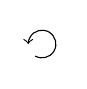
\begin{tikzpicture}[baseline]
    \draw[->](0, 0) arc (-120:180:.5em);
  \end{tikzpicture}
}

\begin{center}
  \begin{tikzcd}[column sep=tiny]
    \widetilde{X}\arrow[d] & \arrow[l, phantom, sloped, "\actson"] G \\ 
    \overline{X} \arrow[d] & \arrow[l, phantom, sloped, "\actson"] G/[G, G] \\ 
    X=S^3-K
  \end{tikzcd}
\end{center}

% \begin{lemma}
%   The following is a short exact sequence of chain complexes
%   \begin{center}
%     \begin{tikzcd}
%       0 \arrow[r] & C_*(\overline{X})\arrow[r, "t-1"] & C_*(\overline{X})\arrow[r] & C_*(X)\arrow[r] & 0 
%     \end{tikzcd}
%   \end{center}
% \end{lemma}
%

A \buff{Seifert surface} $S$ of knot $K$ is an orientable surface with boundary embedded in $S^3$ such that $\partial S=K$. Take a countable amount of $X$, with $S$ without its boundary embedded, and label each with an element from $\Z$. We might now cut each of the copies of $X$ along the Seifert surface of $K$ and identify the $+$ side of $S$ from the $i$-th copy of $X$ with the $-$ side of $S$ from the $(i+1)$-th copy of $X$. Notice that the arising space with a projection to one copy of $X$ is an infinite cyclic cover of $X$.

Imagine that each copy of $X$ inside of $\overline{X}$ is a box labeled with some integer $k$. The ring action of $\Z[\Z]$ on $\overline{X}$ is increasing or decreasing the label on the box from which a cycle is taken, depending on the power of $t\in\Z[\Z]$ in the polynomial which we apply to $\overline{X}$.

\begin{proposition}\label{prop: modul alexandera jest torsyjny}
  The $\Z[\Z]$-module $K^{ab}=H_1(\overline{X}, \Z)$ is a torsion module.
\end{proposition}

\begin{proof}
  Consider the following homomorphism on chain complexes:
  $$f:C_*(\overline{X})\to C_*(\overline{X})$$
  $$f(x)=(1-t)x.$$
  It translates to removing from a cycle in the $(i+1)$-th box a corresponding cycle in the $i$-th box. From this it is an immediate result that $\ker f=0$ and that $\coker f=C_*(X)$ : after gluing all pairs of cycles from two consecutive boxes, the result is easily identified with just one box.

  As a consequence, the following sequence of chain complexes is exact
  \begin{center}
    \begin{tikzcd}
      0\arrow[r] & C_*(\overline{X})\arrow[r, "f"] & C_*(\overline{X})\arrow[r] & C_*(X)\arrow[r] & 0
    \end{tikzcd}
  \end{center}
  and induces an acyclic complex of homology modules
  \begin{center}
    \begin{tikzcd}
      ... \arrow[r] & H_2(X, \Z)\arrow[r] & H_1(\overline{X}, \Z)\arrow[r, "1-t"] & H_1(\overline{X}, \Z)\arrow[r] & H_1(X, \Z)
      \arrow[dlll, rounded corners, to path={--([xshift=2ex]\tikztostart.east) |- ([xshift=-3ex, yshift=-2ex]\tikztostart.south) -| ([xshift=-2ex]\tikztotarget.west) -- (\tikztotarget)
      }]\\ 
                    & H_0(\overline{X}, \Z)\arrow[r] & H_0(\overline{X}, \Z)\arrow[r] & H_0(X, \Z)\arrow[r] & 0
    \end{tikzcd}
  \end{center}
  As was mentioned previously, the following equality holds:
  $$H_1(X, \Z)=\pi_1(X)^{ab}=\Z.$$
  Now, because $X$ is homotopy cycle, then $H_2(X, \Z)=0$. Both $X$ and $\overline{X}$ is connected implying that 
  $$H_0(X, \Z)=H_0(\overline{X}, \Z)=\Z.$$
  \begin{center}
    \begin{tikzcd}
      ... \arrow[r] & 0\arrow[r] & H_1(\overline{X}, \Z)\arrow[r, "1-t"] & H_1(\overline{X}, \Z)\arrow[r, "0"] & \Z \arrow[dlll, "\cong", rounded corners, to path={--([xshift=2ex]\tikztostart.east) |- ([xshift=-3ex, yshift=-2ex]\tikztostart.south) -| ([xshift=-2ex]\tikztotarget.west) -- (\tikztotarget)
      }]\\ 
                    & \Z \arrow[r, "0"] & \Z\arrow[r, "\cong"] & \Z \arrow[r] & 0
    \end{tikzcd}
  \end{center}
  Rewriting the sequence above we easily get that homomorphism $1-t$ is actually an isomorphism and $H_1(\overline{X}, \Z)\cong (1-t) H_1(\overline{X}, \Z)$, which allows us to use the Nakayama's lemma to conclude that there exists $x\in\Z[\Z]$ such that
  $$xH_1(\overline{X}, \Z)=0.$$
\end{proof}
